\bluepage{Primitive Restart Index}

\begin{frame}[fragile]
\frametitle{Primitive restart index}
	\begin{figure}[h]
	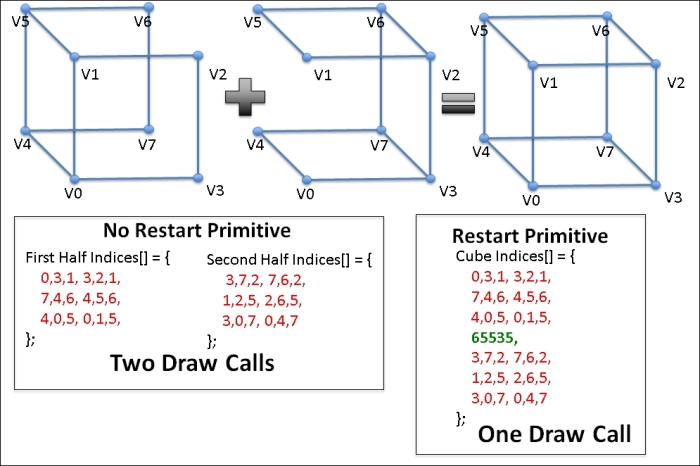
\includegraphics[width=10cm,keepaspectratio]{pics/pri.jpg}
	\end{figure}
\url{https://www.packtpub.com/mapt/book/application_development/9781849695527/3/ch03lvl1sec36/rendering-multiple-primitives-with-primitive-restart}
\end{frame}


\begin{frame}[fragile]
\frametitle{Primitive restart index}
	\begin{itemize}
    \item Primitive restart index can be use to terminated triangle strip.
    \item If we want to draw a lot of triangle strips that are not connected, we can use PRI.
    \item Without PRI, we would have to use glDrawElements for each triangle strip.
    \item or we would have to degenerated some primitives.
    \item PRI is used as element of element array buffer.
    \item Primitive assembly is terminated after reaching PRI.
	\end{itemize}
\begin{minted}[bgcolor=bg]{packages/c_cpp.py:CppLexer -x}
glEnable(GL_PRIMITIVE_RESTART);
glPrimitiveRestartIndex(0xffffffff);
\end{minted}
\end{frame}


